\clearpage
\subsection{Identifier} % (fold)
\label{sub:identifier}

An Identifier is the technical term for the words that \emph{identify} something for the compiler. These can be the \textbf{name} of a programming artefact such as a Program, Library, or Procedure, or the words that have special means for the compiler. You will use Identifiers to name the artefact you create, and to select the appropriate artefact when it is used.

\begin{figure}[h]
   \centering
   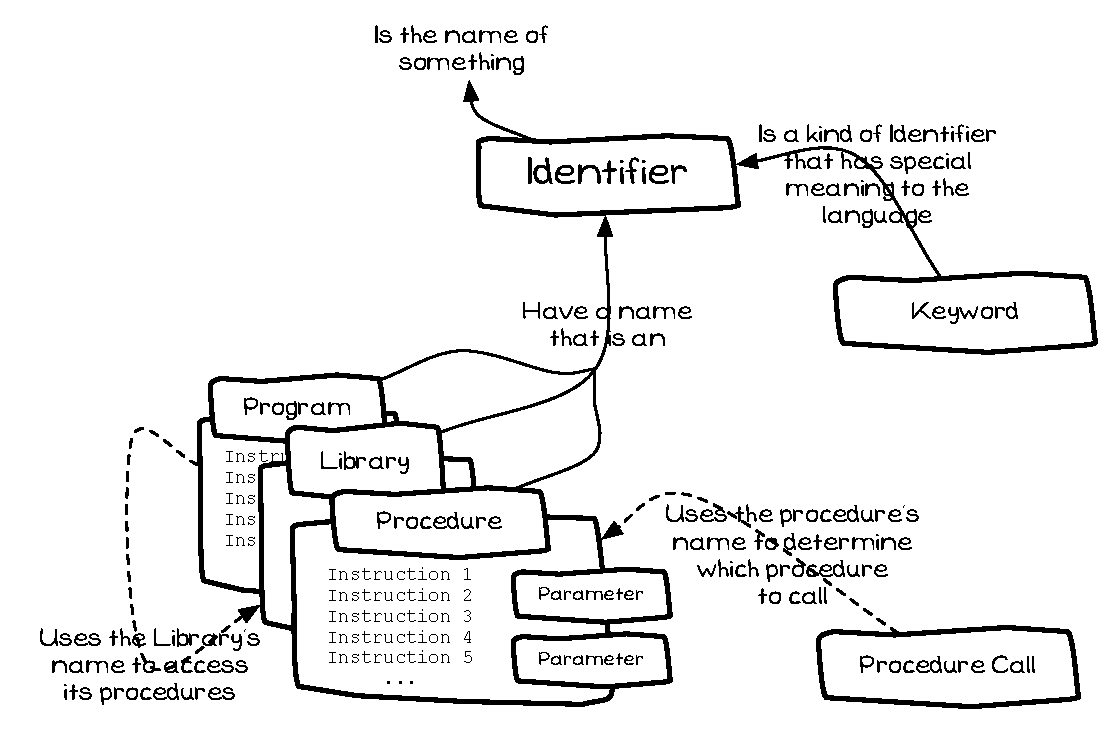
\includegraphics[width=\textwidth]{./topics/program-creation/diagrams/Identifier} 
   \caption[Identifier Concept Diagram]{An Identifier is the name of a programming artefact such as a Program, Library, or Procedure.}
   \label{fig:program-creation-identifier}
\end{figure}


\mynote{
\begin{itemize}
  \item Figure \ref{fig:program-creation-identifier} shows the concepts related to an Identifier.
  \item An Identifier is a \textbf{name} used to identify a programming artefact such as a \nameref{sub:program}, \nameref{sub:library} or \nameref{sub:procedure}.
  \item The name you give your Program is an Identifier.
  \item You use Identifiers to indicate which Libraries you want to access in your Program.
  \item The \nameref{sub:procedure call} uses the Procedure's identifier to determine which procedure is called.
\end{itemize}
}

% section program (end)